\documentclass[runningheads, a4paper]{llncs}

\usepackage[utf8]{inputenc}
\usepackage{hyperref}
\usepackage{graphicx}
\usepackage{listings}

\begin{document}

\title{VirtualSOC}


\author{Socea Teodor}

\authorrunning{Socea T.}

\institute{Universitatea "Alexandru Ioan Cuza", Iași, 
\email{secretariat@info.uaic.ro}\\
\url{https://www.info.uaic.ro}}

\maketitle

\begin{abstract}
The following document contains details about the implementation and functionality of the VirtualSOC project, a client/server application aiming to simulate a social network. In the following sections can be found all possible commands, the message evaluation process and the technologies used.

\keywords{Social Network \and Server \and Client \and TCP/IP}
\end{abstract}

\section{Introduction}
VirtualSOC is an application aiming to simulate a social network. Users will be able to connect to the concurrent VirtualSOC server using the VirtualSOC client. Users will be able to view posts on the network, register for an account or log into an existing one. A registered user can post news and add friends. They can also change their profile to private or post news only a specific group of friends can view.\\
The server can be hosted on any Linux based machine and will run on port 2030 by default, but that can be changed in the code.\\
The client can run on any Linux based machine and provides a user friendly menu based console interface, no GUI is present.

\section{Technologies Used}
\subsection{C++}
The entirety of the application, both the client and the server are written in C++ and are aimed to be used on the Linux operation system exclusively. The reason for choosing to work with C++ over C was a simple one. It provides all the functionality a low level implementation would need but also has higher level features like OOP and templated types such as strings and vectors.
\subsection{TCP/IP}
The app only uses the TCP/IP protocol, because the sent messages from the client or the server need to be intact and in order when they reach. Therefor the correctness of the sent packets was prioritized for determining the memory to be used and the time of execution.\\
In other words, UDP (acronym for \textbf{U}ser \textbf{D}atagram  \textbf{P}rotocol) packet technology is not connection oriented meaning it does not perform checks for a correct transmission of packets and it can lead to incorrect messages sent or lost on the way.\\
On the other hand, the TCP (acronym for \textbf{T}ransfer \textbf{C}ontrol \textbf{P}rotocol)  technology is connection oriented, bringing significant advantages to the application. The packets are sent integrally and in order and a check is always performed when receiving them. Despite the fact that these checks may have an impact on the performance, it is a trade off I was willing to make because having a complete packet is better than an incomplete one.
\subsection{SQLite}
The server side application uses the SQLite library for creating a database to store all the information in. SQLite databases are not "real databases", however they are easy to work with and are interfaced with the SQL language. More about the architecture of the database can be found further in the document.
\subsection{OpenSSL}
The client side application uses the OpenSSL library for hashing the user passwords. The aim of this was to hash the password as soon as possible and send it over the network already hashed, so anyone trying to capture information on the network will be unable to get the password. The SHA256 algorithm was chosen because it is fairly fast and incredibly difficult to brute force back to the original.  On top of that, both the client and server side applications use a base64 encoding mechanism to encode and decode data sent over the network, so that no unexpected characters are present in parsing the package received.
\section{Architecture}
\subsection{Application Diagram}
The application contains 3 components that communicate with each other: Client - Server and Server - Database. For efficiency, a concurrent server was implemented, using the \texttt{fork()} function in order to create child processes which will handle each client request.
\newpage
\begin{figure}[h!]
    \centering
    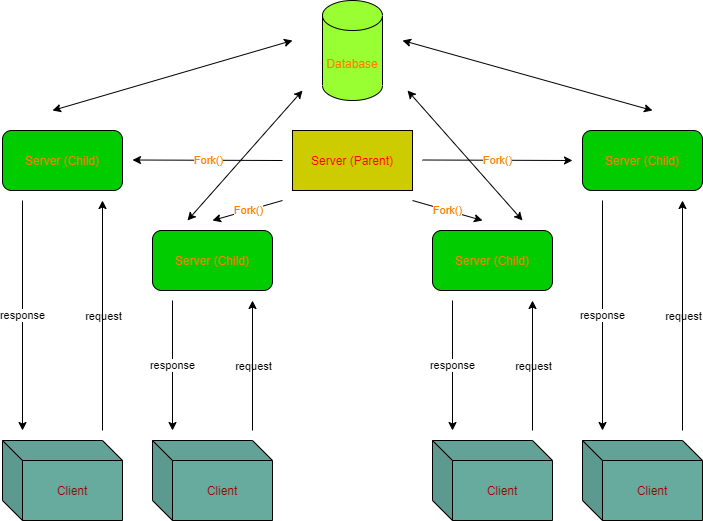
\includegraphics[width=13cm, height=10cm, keepaspectratio]{Archt.png}
    \caption{Application Architecture}
    \label{funct:diagram}
\end{figure}
\subsection{Data structures used}
The application uses the following data structures in the form of classes:
\begin{itemize}
    \item The $Command$ class used for storing elements of a command to be sent to the server. 
    \begin{lstlisting}
    class Command {
        string id;
        vector<string> args;
    }
    \end{lstlisting}
    \item  The $Response$ class used for storing elements of a response to be sent to the client.
    \begin{lstlisting}
    class Response {
        string status;
        vector<string> args;
    }
    \end{lstlisting}
    \item The $Post$ class used for storing elements of a post. Certain elements of a post will be sent and received as arguments for $Commands$ or $Responses$.
    \begin{lstlisting}
    class Post {
        int id;
        string title;
        string author;
        string content;
        string date;
        string type;
    }
    \end{lstlisting}
    \item The $User$ class used for consistency between the server and client. Users can be of type "REGULAR" or "ADMIN".
    \begin{lstlisting}
    class User{
        int id;
        string username;
        string type;
    }
    \end{lstlisting}
\end{itemize}

\subsection{Database Architecture}
The server side application uses a SQLite database, as previously stated, because of how simple and efficient it is to work with. So far the database has 3 tables: Users, Posts and Friends.\\
The Users table stores information about the users such as the Username, Password and Type. The password represents the hashed passwords the user has registered with. The type can be REGULAR or ADMIN.\\
The Posts table stores all the posts REGULAR users have created. Posts have a Title, Author, Content, Type and Date. The Date is the moment the post was created and is stored in unix time. The Type of a post can be PUBLIC, FRIENDS or FAMILY.\\
The Friends table stores the ID's of REGULAR users who are friends with each other and the Type of friends they are, like FRIENDS or FAMILY.\\
Message storage is handled by the database using tables whose names respect the following naming schema : "TBmin(id1, id2)$__$max(id1, id2)". and store the sender, the message itself and the timestamp of when the message has reached the server.\\
\begin{figure}
    \centering
    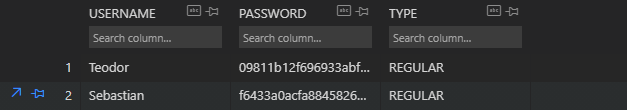
\includegraphics[width = 10cm, height = 5cm, keepaspectratio]{Users.PNG}
    \caption{Users Table}
\end{figure}
\begin{figure}
    \centering
    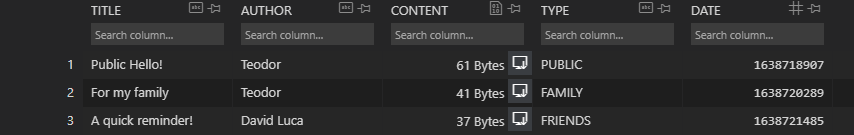
\includegraphics[width = 10cm, height = 5cm, keepaspectratio]{Posts.PNG}
    \caption{Posts Table}
\end{figure}
\begin{figure}
    \centering
    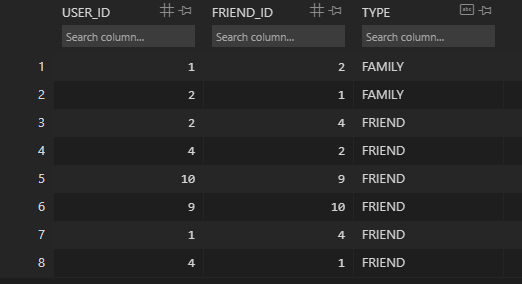
\includegraphics[width = 10cm, height = 5cm, keepaspectratio]{Friends.PNG}
    \caption{Friends Table}
\end{figure}
\begin{figure}
    \centering
    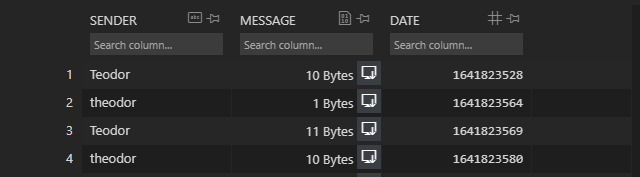
\includegraphics[width = 10cm, height = 5cm, keepaspectratio]{Capture.PNG}
    \caption{Messages Table Example}
\end{figure}
\newpage{}
\section{Implementation Details}
In the following sections can be found a description of the protocol used in the application and how the messages are being sent between the client and the server.
Possible situations:
\begin{itemize}
    \item A client has connected to the server as guest.\\
    The guest has access to the following commands:
    \begin{itemize}
        \item \texttt{register} $\rightarrow$ after the registration process, a message respecting the folling format will be created: \texttt{REGISTER:USERNAME:PASSWORD}, where the password is already hashed. These are the following responses the server will send:
        \begin{itemize}
            \item \texttt{SUCCESS} $\rightarrow$ registration completed successfully
            \item \texttt{FAILED:USERNAME ALREADY EXISTS} $\rightarrow$ registration did not complete successfully because the username already exists
        \end{itemize}
        \item \texttt{login} $\rightarrow$ after the login process the following message will be constructed: \texttt{LOGIN:USERNAME:PASSWORD}. These are the responses the server will send:
        \begin{itemize}
            \item \texttt{SUCCESS} $\rightarrow$ loged in successfully
            \item \texttt{FAILED:WRONG PASSWORD} $\rightarrow$ username or password wrong
            \item \texttt{FAILED:USERNAME DOES NOT EXIST} $\rightarrow$ the username does not exist in the database
        \end{itemize}
        \item \texttt{View Posts} $\rightarrow$ is the method guest users can see the public posts on the network. A message like \texttt{LOOKUP:PUBLIC} will be sent, which will receive the following response:
        \begin{itemize}
            \item \texttt{SUCCESS:POSTCOUNT} $\rightarrow$ the server will send the client POSTCOUNT posts in forms of strings.
            \item \texttt{NOPOSTS} $\rightarrow$ no more posts are available to view
        \end{itemize}
        \item \texttt{Close Application} $\rightarrow$ this will terminate the connectiont to the server.
    \end{itemize}
    \hfill \\
    \item The client has connected as \textbf{REGULAR} to the server. \\
    These are the available commands:
    \begin{itemize}
        \item \texttt{View Posts} $\rightarrow$ the REGULAR user will send messages representing which type of posts they would like to see like GETPOSTS:PUBLIC, GETPOSTS:FRIENDS, GETPOSTS:FAMILY and will receive the same response as a guest user with filtered posts.
        \item \texttt{Add Friend} using this command users can add friends to their friends list. LOOKUP:FRIENDUSERNAME will be sent to the server. The server will send back a list of users that match the FRIENDUSERNAME sent. The authenticated user can select a username and the type and send to the server ADDFRIEND:USERNAME:TYPE.
        \item \texttt{Create Post} $\rightarrow$ Using this command the user can create a post, give it a title and select what group the post is adressed to. After this process is completed, the message will be created: \\CREATEPOST:TITLE:CONTENT:TYPE. \\The server will send a SUCCESS response regardless of if it errored or not.
        \item \texttt{View Friends} $\rightarrow$ Using this command the user can view their friends list. The message sent to the server is LOOKUP:FRIENDS. The server will return the message SUCCESS:FRIENDSCOUNT, followed by \\FRIEND:USERNAME - TYPE, or NOFRIENDS when no friends are available. If a friend from the list is selected the client will send a CHATWITH:FRIENDNAME message to the server and will begin chatting with that person. The server will send SUCCESS:MESSAGECOUNT and the latest 10 messages in the table as MESSAGE:MESSAGECONTENT. The user can press "ESC" to send DONE to the server and return to the main menu.
        \item \texttt{Log out} $\rightarrow$ Using this command the user will log out and become a guest user. Message is : LOGOUT. Server will send back SUCCESS.
        \item \texttt{Close Application} $\rightarrow$ The client is going to send QUITSESSION to the server and close. The server will exit out of the child.
    \end{itemize}
    \hfill \\
    \item The client has connected to the server using an \textbf{ADMIN} account. \\
    An administrator only has access to 3 commands:
    \begin{itemize}
        \item \texttt{Delete Posts} $\rightarrow$ Using the same protocol for getting posts previously mentioned, the user will receive a list of all posts, public or private, and will be able to select one and delete it. The delete command is DELETE:POSTID. The server will respond with SUCCESS regardless.
        \item \texttt{Log out} Is the same like a REGULAR user.
        \item \texttt{Close Application} Is the same like a REGULAR user.
    \end{itemize}
\end{itemize}
\newpage
\section{Conclusions}
At the moment the application is working as intended, the commands and messages are parsed accordingly, and the user interface is intuitive and easy to use, however there are a few improvements that can be made.\\ First of all, message security was not prioritized so they are sent as base64 encoded text over the network, adding a layer of inconvenience to an attacker. \\
The application does support a messaging feature however there are no automatic refreshes. This could be improved and turned into a live chat.
Lastly, further ADMIN functionalities could be implemented such as a shut down remotely.
\begin{thebibliography}{}
\bibitem{course}
Retele de Calculatoare\\
\url{https://profs.info.uaic.ro/~computernetworks/}

\bibitem{stackoverflow}
StackOverflow \\
\url{https://stackoverflow.com}

\bibitem{tex}
Tex StackExchange \\
\url{https://tex.stackexchange.com/}

\bibitem{diagram}
Diagram Software and Flowchart Maker \\
\url{https://www.diagrams.net/}
\bibitem{TutorialsPoint}
TutorialsPoint\\
\url{https://www.tutorialspoint.com/index.html}
\end{thebibliography}
\end{document}
